%%%%%%%%%%%%%%%%%%%%%%%%%%%%%%%%%%%%%%%%% 
% Journal Article
% LaTeX Template
% Version 1.3 (9/9/13)
% 
% This template has been downloaded from:
% http://www.LaTeXTemplates.com
% 
% Original author:
% Frits Wenneker (http://www.howtotex.com)
% 
% License:
% CC BY-NC-SA 3.0 (http://creativecommons.org/licenses/by-nc-sa/3.0/)
% 
%%%%%%%%%%%%%%%%%%%%%%%%%%%%%%%%%%%%%%%%% 

% ----------------------------------------------------------------------------------------
%	PACKAGES AND OTHER DOCUMENT CONFIGURATIONS
% ----------------------------------------------------------------------------------------

\documentclass[twoside]{article}

\usepackage{lipsum} % Package to generate dummy text throughout this template

\usepackage[sc]{mathpazo} % Use the Palatino font
\usepackage[T1]{fontenc} % Use 8-bit encoding that has 256 glyphs
\linespread{1.05} % Line spacing - Palatino needs more space between lines
\usepackage{microtype} % Slightly tweak font spacing for aesthetics

\usepackage[hmarginratio=1:1,top=32mm,columnsep=20pt]{geometry} % Document margins
\usepackage{multicol} % Used for the two-column layout of the document
\usepackage[hang, small,labelfont=bf,up,textfont=it,up]{caption} % Custom captions under/above floats in tables or figures
\usepackage{booktabs} % Horizontal rules in tables
\usepackage{float} % Required for tables and figures in the multi-column environment - they need to be placed in specific locations with the [H] (e.g. \begin{table}[H])
\usepackage{hyperref} % For hyperlinks in the PDF

\usepackage{lettrine} % The lettrine is the first enlarged letter at the beginning of the text
\usepackage{paralist} % Used for the compactitem environment which makes bullet points with less space between them

\usepackage{abstract} % Allows abstract customization
\renewcommand{\abstractnamefont}{\normalfont\bfseries} % Set the "Abstract" text to bold
\renewcommand{\abstracttextfont}{\normalfont\small\itshape} % Set the abstract itself to small italic text

\usepackage{titlesec} % Allows customization of titles
\renewcommand\thesection{\Roman{section}} % Roman numerals for the sections
\renewcommand\thesubsection{\Roman{subsection}} % Roman numerals for subsections
\titleformat{\section}[block]{\large\scshape\centering}{\thesection.}{1em}{} % Change the look of the section titles
\titleformat{\subsection}[block]{\large}{\thesubsection.}{1em}{} % Change the look of the section titles

\usepackage{fancyhdr} % Headers and footers
\pagestyle{fancy} % All pages have headers and footers
\fancyhead{} % Blank out the default header
\fancyfoot{} % Blank out the default footer
\fancyhead[C]{CDNLive Shanghai $\bullet$ Auguset 2015 $\bullet$ Vol. XXX, No. X} % Custom header text
\fancyfoot[RO,LE]{\thepage} % Custom footer text

\usepackage{graphicx}
\usepackage{multirow}
\graphicspath{ {images/} }

% ----------------------------------------------------------------------------------------
%	TITLE SECTION
% ----------------------------------------------------------------------------------------

\title{\vspace{-15mm}\fontsize{24pt}{10pt}\selectfont\textbf{Compilation and Elaboration Speeding Up and Space Saving by Pre-Compilation, MSIE and Parallel Processing Technology}} % Article Title
\author{
  \large
  \textsc{Guanyu Yi}\thanks{Special thanks for the help and support of Liang Chen from Cadence}, \textsc{Rosemary Hu}, \textsc{Gary Gao} \\[2mm]
  \textsc{Jianhong Chen}, \textsc{Weitao Wang}, \textsc{Richard Sun}, \textsc{Johnny Li} \\[2mm] % Your name
  \normalsize Spreadtrum Communications, Inc. \\ % Your institution
  \normalsize \href{mailto:guanyu.yi@spreadtrum.com}{guanyu.yi@spreadtrum.com} % Your email address
  \vspace{-5mm}
}
\date{}

% ----------------------------------------------------------------------------------------

\begin{document}
\maketitle % Insert title
\thispagestyle{fancy} % All pages have headers and footers

% ----------------------------------------------------------------------------------------
%	ABSTRACT
% ----------------------------------------------------------------------------------------

\begin{abstract}

  With technology node shrinks further, we are seeing more and more billion gate design in production, and 10 billion gate design is no impossible. But the bigger design size is, the exponentially slower functional verification turn around becomes. Without innovative technology, even one small testcase or design change would take a full day to compile and elaborate, not to mention the unexpected typo might be found late in the cycle. In Spreadtrum, we are dealing with the several complicated AP SOC designs at the same time, the time to market restriction enforce us to look for some advanced technologies that could help us shorten the turn around time while maintaining the same verification quality. Cadence Incisive Enterprise Simulator comes with pre-compiled libraries feature and multiple snapshot incremental elaboration technology, combine both technologies help us to reduce the clean build time into 1/6 of the original, and the build time of single testcase change could be reduced to less than 10 minutes. With these technologies, we are not only speed up the debug turn around time, but also suffer less from the turbulence of the IT infrastructure.

\end{abstract}

% ----------------------------------------------------------------------------------------
%	ARTICLE CONTENTS
% ----------------------------------------------------------------------------------------

\begin{multicols}{2} % Two-column layout throughout the main article text

  \section{Introduction}

  \lettrine[nindent=0em,lines=3]{N}owadays, VLSI is developing more and more rapidly. Billions of gates included in ASIC design is more and more common, especially for large scale of SoC design team.

  The advantage of this fast developed technology mainly consists of the smaller size and lower power consumption. The chip size and power consumption reduction of chips makes them be easily integrated together into smaller SoC, which can be used by hardware companies, such as Apple, Sumsung, Lenovo, etc., to invent fascinating mature electronic productions to bring improvement even evolution to our daily life.
  
  However, each coin has two sides, the dark side is the challenge of simulation tools, which is required to be more powerful to handle such large scale of gate design. According to the simulation data statistics by Cadence before, the pure simulation and elaboration time of one small testcase will take a full day on the billions of gates SoC design. Moreover, current mature project needs test case regression system to kick off thousands of test cases to make sure the RTL design modification during a period of time is correct. The pure space occupied by compiled libraries of each case is several gigabytes large, and only one time of regression will take several terabytes. Considering we have dozens of projects running in parallel and one or two times of regression each week, the disk space occupation is too large to ignore the influence. So the innovative technology is necessary to speed up our simulation and elaboration processes and to save the simulation space occupation.

  % ------------------------------------------------

  \section{Methods}

  Taking the ease of usage in the industry into consideration, we choose the parallel processing as the speeding up method and libraries reuse as the space saving method.

  Parallel computing is a form of computation in which many calculations are carried out simultaneously.\cite{parallel} Parallel processing can be performed by multi-threading, multi-processing or Platform Load Sharing Facility(\textbf{LSF}) technologies. In Spreadtrum Communications, Inc.(\textbf{SPRD}) production environment, it is convenient to use LSF, which can be used to execute batch jobs on networked Unix and Windows systems on many different architectures,\cite{LSF1}\cite{LSF2} as the core called part and to use multi-processing module as the interface calling part.

  Cadence simulation tool provides two wonderful technologies for shared libraries reuse, which are called pre-compilation and multi-snapshot incremental elaboration(\textbf{MSIE}).

  The former is that you can pre-compile files into a library with the -compile and -makelib options, and then reference the library with the -reflib option for elaboration. The latter provides a form of incremental elaboration that can greatly decrease the time it takes to re-elaborate a design.

  As we already know, the entire RTL design can be separated into relatively independent parts according to RTL design hierarchy of full chip, so we can make good use of the boundaries of each sub system to building each parts into each snapshots. Meanwhile, we can collect some commonly used modules such as tech libraries and IPs into shared libraries for being referred to by each snapshots. The former technology is MSIE, while the latter technology is pre-compilation.

  Pre-compilation and MSIE can be used together with parallel processing to achieve our goal to speed up compilation and elaboration and to save space used by test cases

  Suppose we have a RTL design called DUT and a test bench called TB. We will compile DUT, which is the largest time and space consuming part, into several sets of modules called libraries. Each library has its own property, such as IP library, standard cell library, vhdl module library, etc., and these property separated libraries can be reused to building elaborated snapshots. Assuming the DUT is split into three main sub systems according to different features, such as application processing sub system, communication processing sub system, multimedia processing sub system, etc., and each sub system can be elaborated as a snapshot by referring to the pre-compiled libraries. The detailed mapping relationship is shown in the Figure \ref{fig:pm_mapping}.
  \begin{figure}[H]
    \centering
    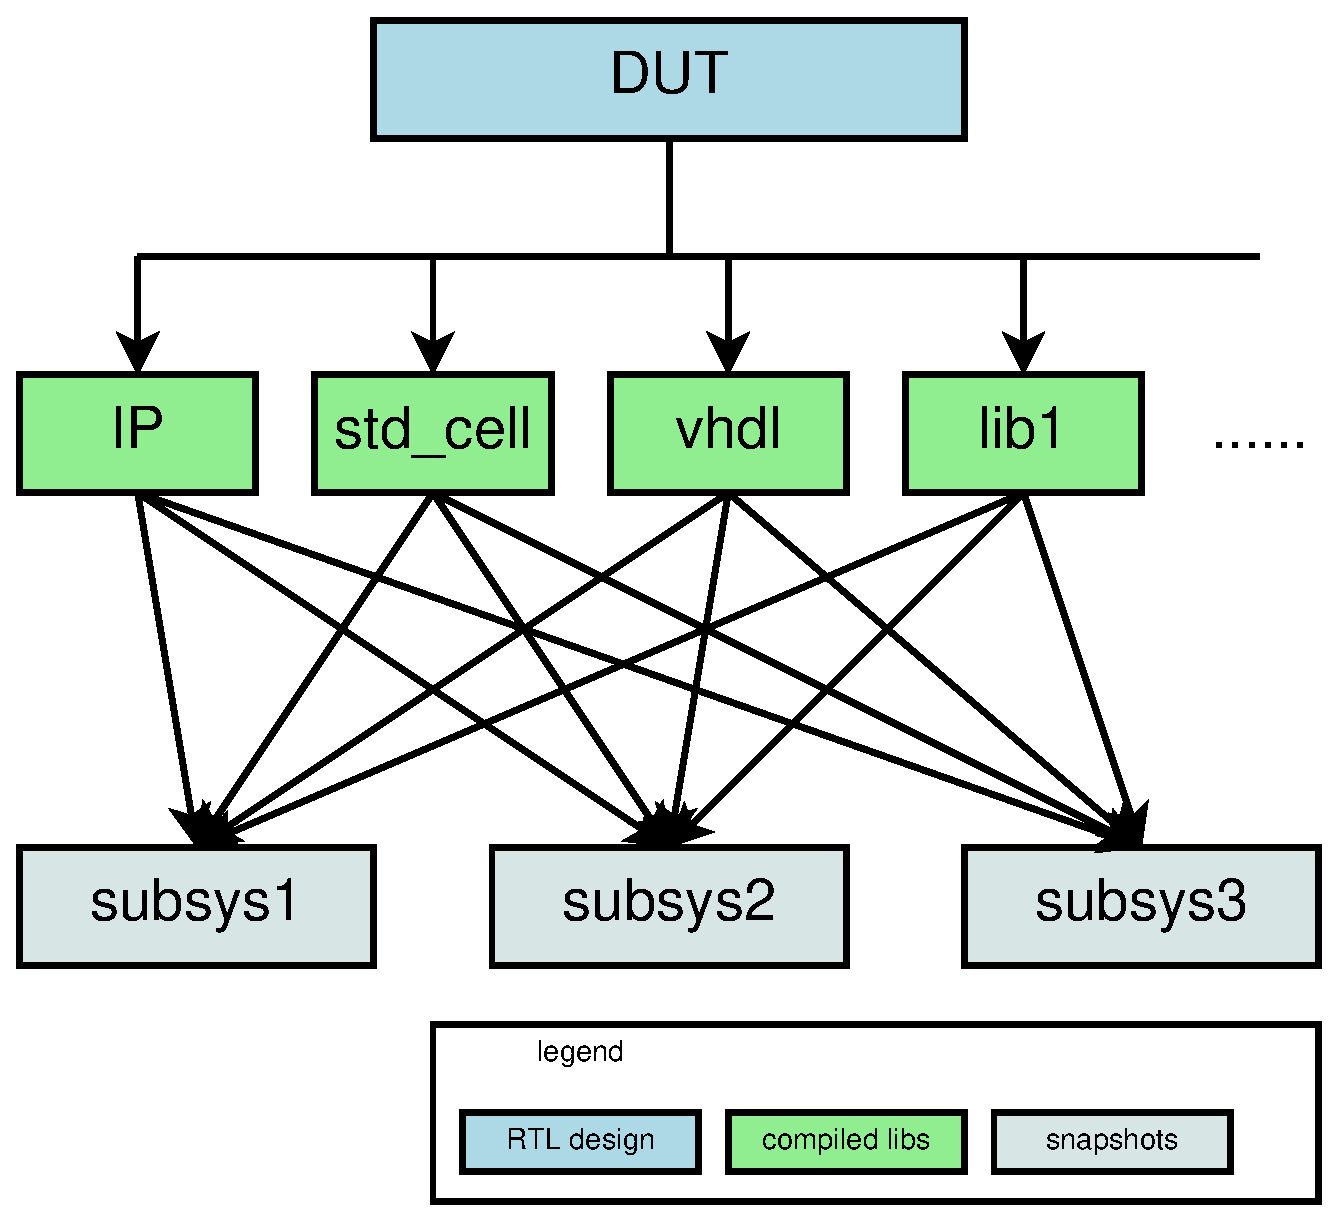
\includegraphics[width=\linewidth]{pm_mapping}
    \caption{libraries and snapshots mapping}
    \label{fig:pm_mapping}
  \end{figure}

  The stage of splitting DUT into compiled libraries is called pre-compilation, and the stage of referring to all libraries to do elaboration of each sub systems is called MSIE. With these Cadence technologies, we can reuse the libraries or snapshots for each regression case to reduce the space usage dramatically.

  During pre-compilation and MSIE stages, multi-processing and LSF parallel technologies can be used to reduce the compilation and elaboration time, which is shown in the Figure \ref{fig:parallel}.
  \begin{figure}[H]
    \centering
    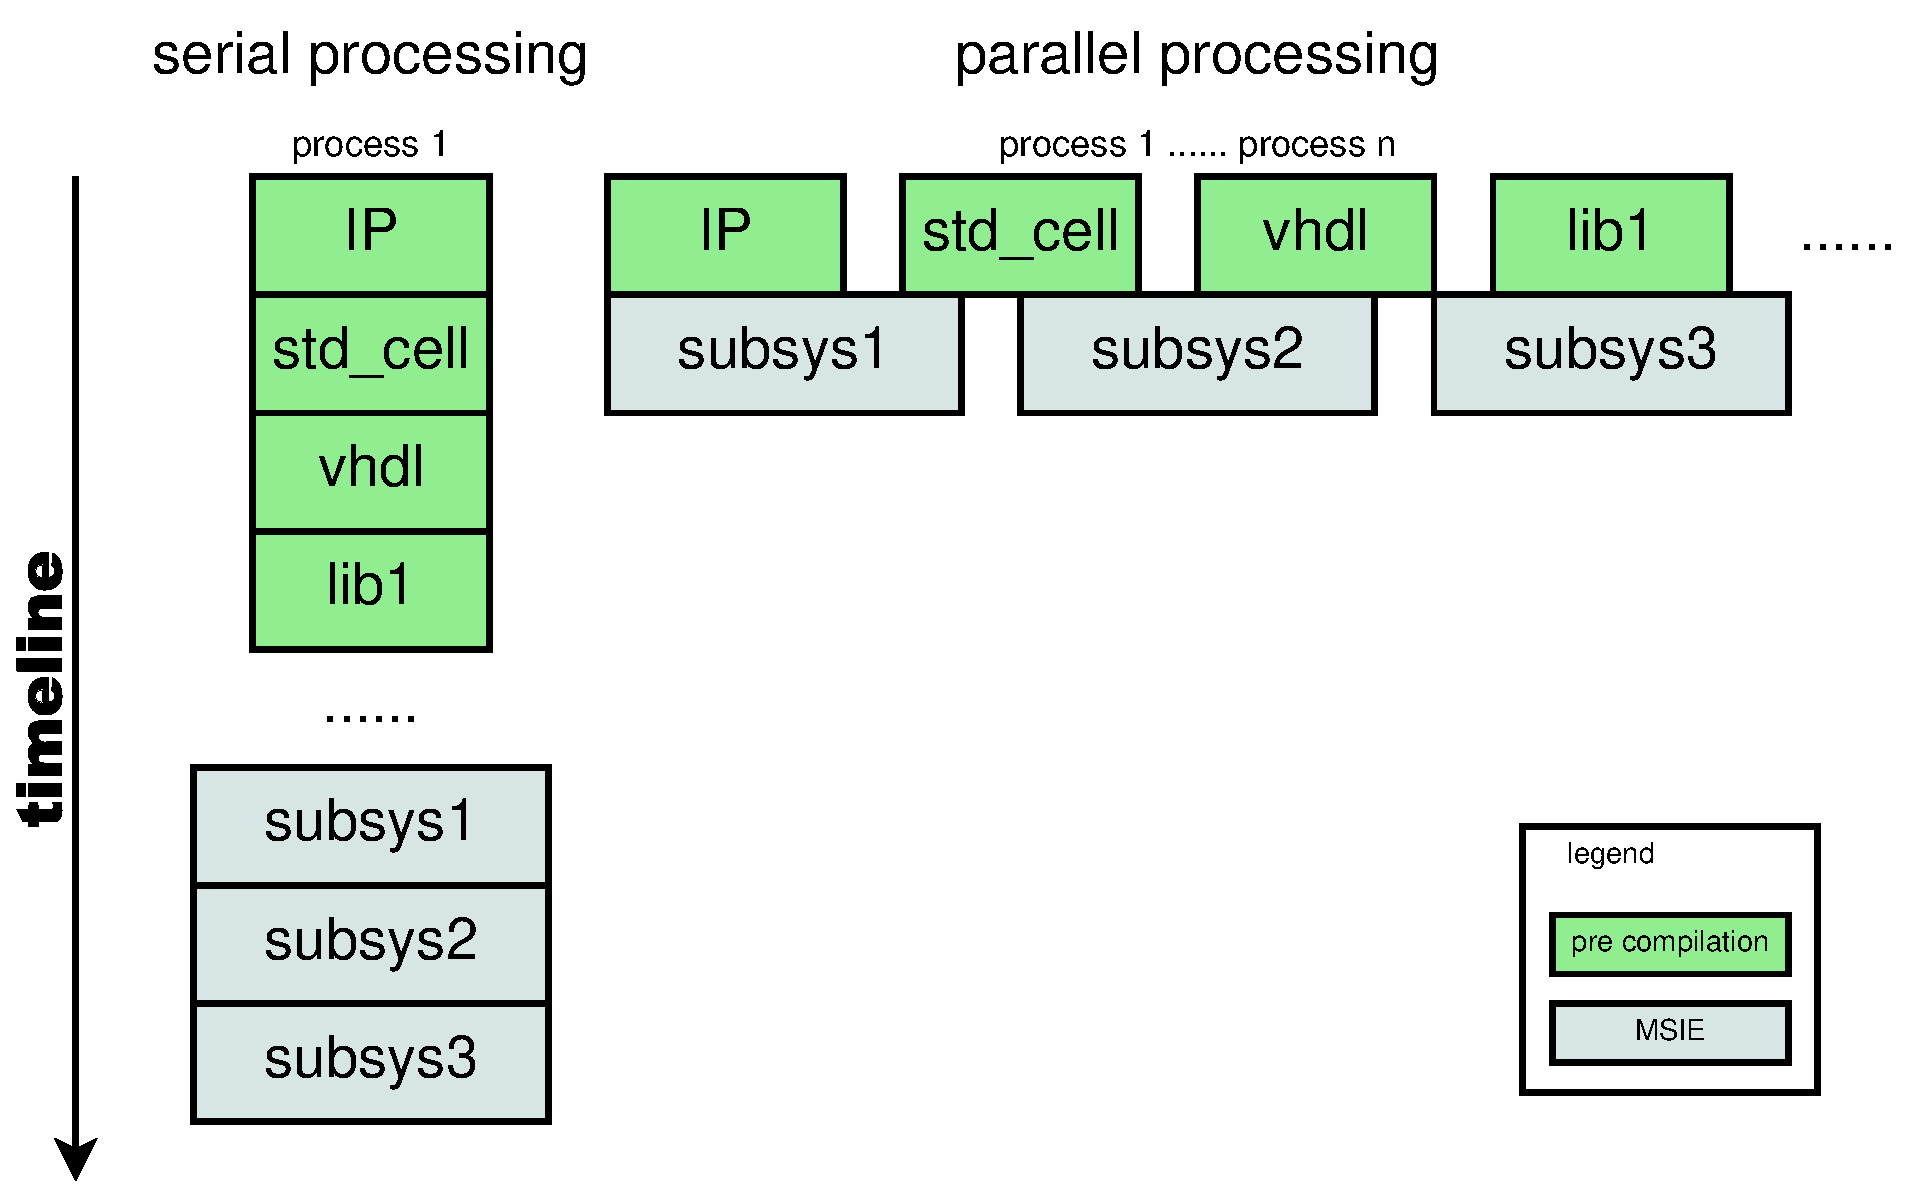
\includegraphics[width=\linewidth]{parallel}
    \caption{parallel processing}
    \label{fig:parallel}
  \end{figure}
  Since the compilation and elaboration time is much more important than the CPU resources of LSF, we take this time-resource trade-off of costing more CPU resources to save time.

  % ------------------------------------------------

  \section{Results}

  In this section, we will take the \textbf{empty} case from a project of SPRD as the example to demonstrate the speeding up and space saving technology.
  
  In SPRD test case experience, the simulation calling routine is performed by prun written in python, and the indexing parallel processing is done by multiprocessing module. Prun handles parallel processing using pre-compilation, MSIE and LSF and finally calls irun for compilation and elaboration.

  There are mainly 5 steps to implement compilation and elaboration using prun:
  \begin{compactitem}
  \item pre compilation to split DUT into separated libraries
  \item MSIE elaboration to build DUT into separated sub system snapshots
  \item test case href file generation for MSIE reuse, it can be split into two detailed steps for multiple case href files generation together
    \begin{compactitem}
    \item generating all href files for all test cases
    \item collecting and merging all href files together according to sub system
    \end{compactitem}
  \item re-elaboration all the snapshots with generated href files
  \item incremental elaboration the TB with all the sub system snapshots, which is ready to use by simulation
  \end{compactitem}

  Actually each sub system has 3 types of snapshots to build for industry usage, however, more details of this python implementation is omitted here due to the confidential reason. The final time and space consumption comparison results of this experience is shown in the Table \ref{table: time_result} and Table \ref{table: space_result}.

  \begin{table}[H]
    \caption{time comparison table}
    \centering
    \begin{tabular}{lll}
      \toprule
      \textbf{steps} & \textbf{new flow} & \textbf{legacy flow} \\
      \midrule
      pre comp & 1 min 12 sec* & \multirow{5}{*}{23 min 22 sec} \\
      \cline{1-2}
      MSIE elab & 2 min 23 sec* & \\
      \cline{1-2}
      href gen & 2 min 29 sec* & \\
      \cline{1-2}
      re elab & 2 min 29 sec* & \\
      \cline{1-2}
      inc elab & 2 min 16 sec & \\
      \hline
      total & 2 min 16 sec & 23 min 22 sec \\
      \bottomrule
      \multicolumn{3}{l}{\footnotesize{* the time marked star is shared by every case}}
    \end{tabular}
    \label{table: time_result}
  \end{table}

  \begin{table}[H]
    \caption{space comparison table}
    \centering
    \begin{tabular}{lll}
      \toprule
      \textbf{steps} & \textbf{new flow} & \textbf{legacy flow} \\
      \midrule
      pre comp & 4.3 G* & \multirow{5}{*}{5.5 G} \\
      \cline{1-2}
      MSIE elab & \multirow{3}{*}{8.7 G*} & \\
      \cline{1-1}
      href gen & & \\
      \cline{1-1}
      re elab & & \\
      \cline{1-2}
      inc elab & 0.2 G & \\
      \hline
      total & 0.2 G & 5.5 G \\
      \bottomrule
      \multicolumn{3}{l}{\footnotesize{* the space marked star is shared by every case}}
    \end{tabular}
    \label{table: space_result}
  \end{table}

  Using pre-compilation, MSIE and parallel processing technologies, the new flow much faster than legacy flow for a single test case. In the situation of regression, the href files and MSIE snapshots are stable for every case to use, and each case only takes about 2 minutes for incremental elaboration, which is more than 11 times faster than the legacy flow. Moreover, according to the space comparison results shown in the Table \ref{table: space_result}, the space usage is about 30 times less than the legacy flow. The new flow has the tremendous improvement both on the time and space consumption.

  The above part is the data statics of RTL level simulation. Considering the time and space consumption in gate level simulation (\textbf{GLS}) is more horrible than RTL level, and GLS DUT is too stable to re-elaborate snapshots, we also have an experiment of pre-compilation, MSIE and parallel processing in GLS. The Table and Table show the final results.

  \begin{table}[H]
    \caption{GLS time comparison table}
    \centering
    \begin{tabular}{lll}
      \toprule
      \textbf{steps} & \textbf{new flow} & \textbf{legacy flow} \\
      \midrule
      pre comp & 15 min 12 sec* & \multirow{3}{*}{255 min 22 sec} \\
      \cline{1-2}
      MSIE elab & 48 min 15 sec* & \\
      \cline{1-2}
      inc elab & 58 min 33 sec & \\
      \hline
      total & 58 min 33 sec & 255 min 22 sec \\
      \bottomrule
      \multicolumn{3}{l}{\footnotesize{* the time marked star is shared by every case}}
    \end{tabular}
    \label{table: gls_time_result}
  \end{table}

  \begin{table}[H]
    \caption{GLS space comparison table}
    \centering
    \begin{tabular}{lll}
      \toprule
      \textbf{steps} & \textbf{new flow} & \textbf{legacy flow} \\
      \midrule
      pre comp & 4.3 G* & \multirow{3}{*}{15 G} \\
      \cline{1-2}
      MSIE elab & 8.7 G* & \\
      \cline{1-2}
      inc elab & 8.1 G & \\
      \hline
      total & 8.1 G & 15 G \\
      \bottomrule
      \multicolumn{3}{l}{\footnotesize{* the space marked star is shared by every case}}
    \end{tabular}
    \label{table: gls_space_result}
  \end{table}

  In GLS scenario, Using pre-compilation, MSIE and parallel processing technologies, the new flow is about 4 times faster and about 2 times less space consumption than the legacy flow. Since the GLS time and consumption is extremely huge, the new flow has also performed the outstanding contribution.

  % ------------------------------------------------

  \section{Discussion}

  \subsection{Href Files Handling}

  As we may have noticed, the most complex part during the 5 main steps in the advanced flow is the href files handing. 3 out of 5 steps are about that. Principally the href files are used by simulation tool to get the hierarchy permissions during the linking stage, and the file content is based on the test case structure and reference. The simulation tool cannot make sure the permission during compilation, and if taking all hierarchy into consideration, the elaboration efficiency will be reduced dramatically. Cadence has provided an option -primhrefupdate to simplify this complex process, which will re-elaborating the snapshots back automatically for end-user. In regression scenario, since writing back to the same snapshot simultaneously is not possible, we did a trade off and chose the flexible way.

  \subsection{Verilog Configuration Simplicity}

  Referring to multiple libraries sometimes cause an issue that the multiple defined modules need to be resolved due to the referring conflict, which is not a tool issue but related to the RTL design. A straightforward method is to use the standard verilog configuration to define the priority of referring order, which is much more of easy use that the binding option. There is a trouble that the configuration file need to be an extra file and its extension name need to be registered in simulation tools. A solution provided by Cadence is to use the option -libmap which needs only the library referring order, that is more friendly for end-users.

  % ----------------------------------------------------------------------------------------
  %	REFERENCE LIST
  % ----------------------------------------------------------------------------------------

  \begin{thebibliography}{99} % Bibliography - this is intentionally simple in this template

  \bibitem{parallel}
    Gottlieb, Allan; Almasi, George S. (1989).
    Highly parallel computing.
    Redwood City, Calif.: Benjamin/Cummings. ISBN 0-8053-0177-1.

  \bibitem{LSF1}
    Michael R. Ault, Mike Ault, Madhu Tumma, and Ranko Mosic (2004).
    Oracle 10g Grid \& Real Application Clusters.
    Rampant TechPress. p. 24. ISBN 9780974435541.

  \bibitem{LSF2}
    Goering, Richard (March 8, 1999).
    "Load sharing brings kudos".
    EE Times Online. Retrieved 2007-11-12.

  \end{thebibliography}

  % ----------------------------------------------------------------------------------------

\end{multicols}

\end{document}

%%% Local Variables:
%%% mode: latex
%%% TeX-master: t
%%% End:
